\section{Introduction}
\begin{figure*}[t]
\centering
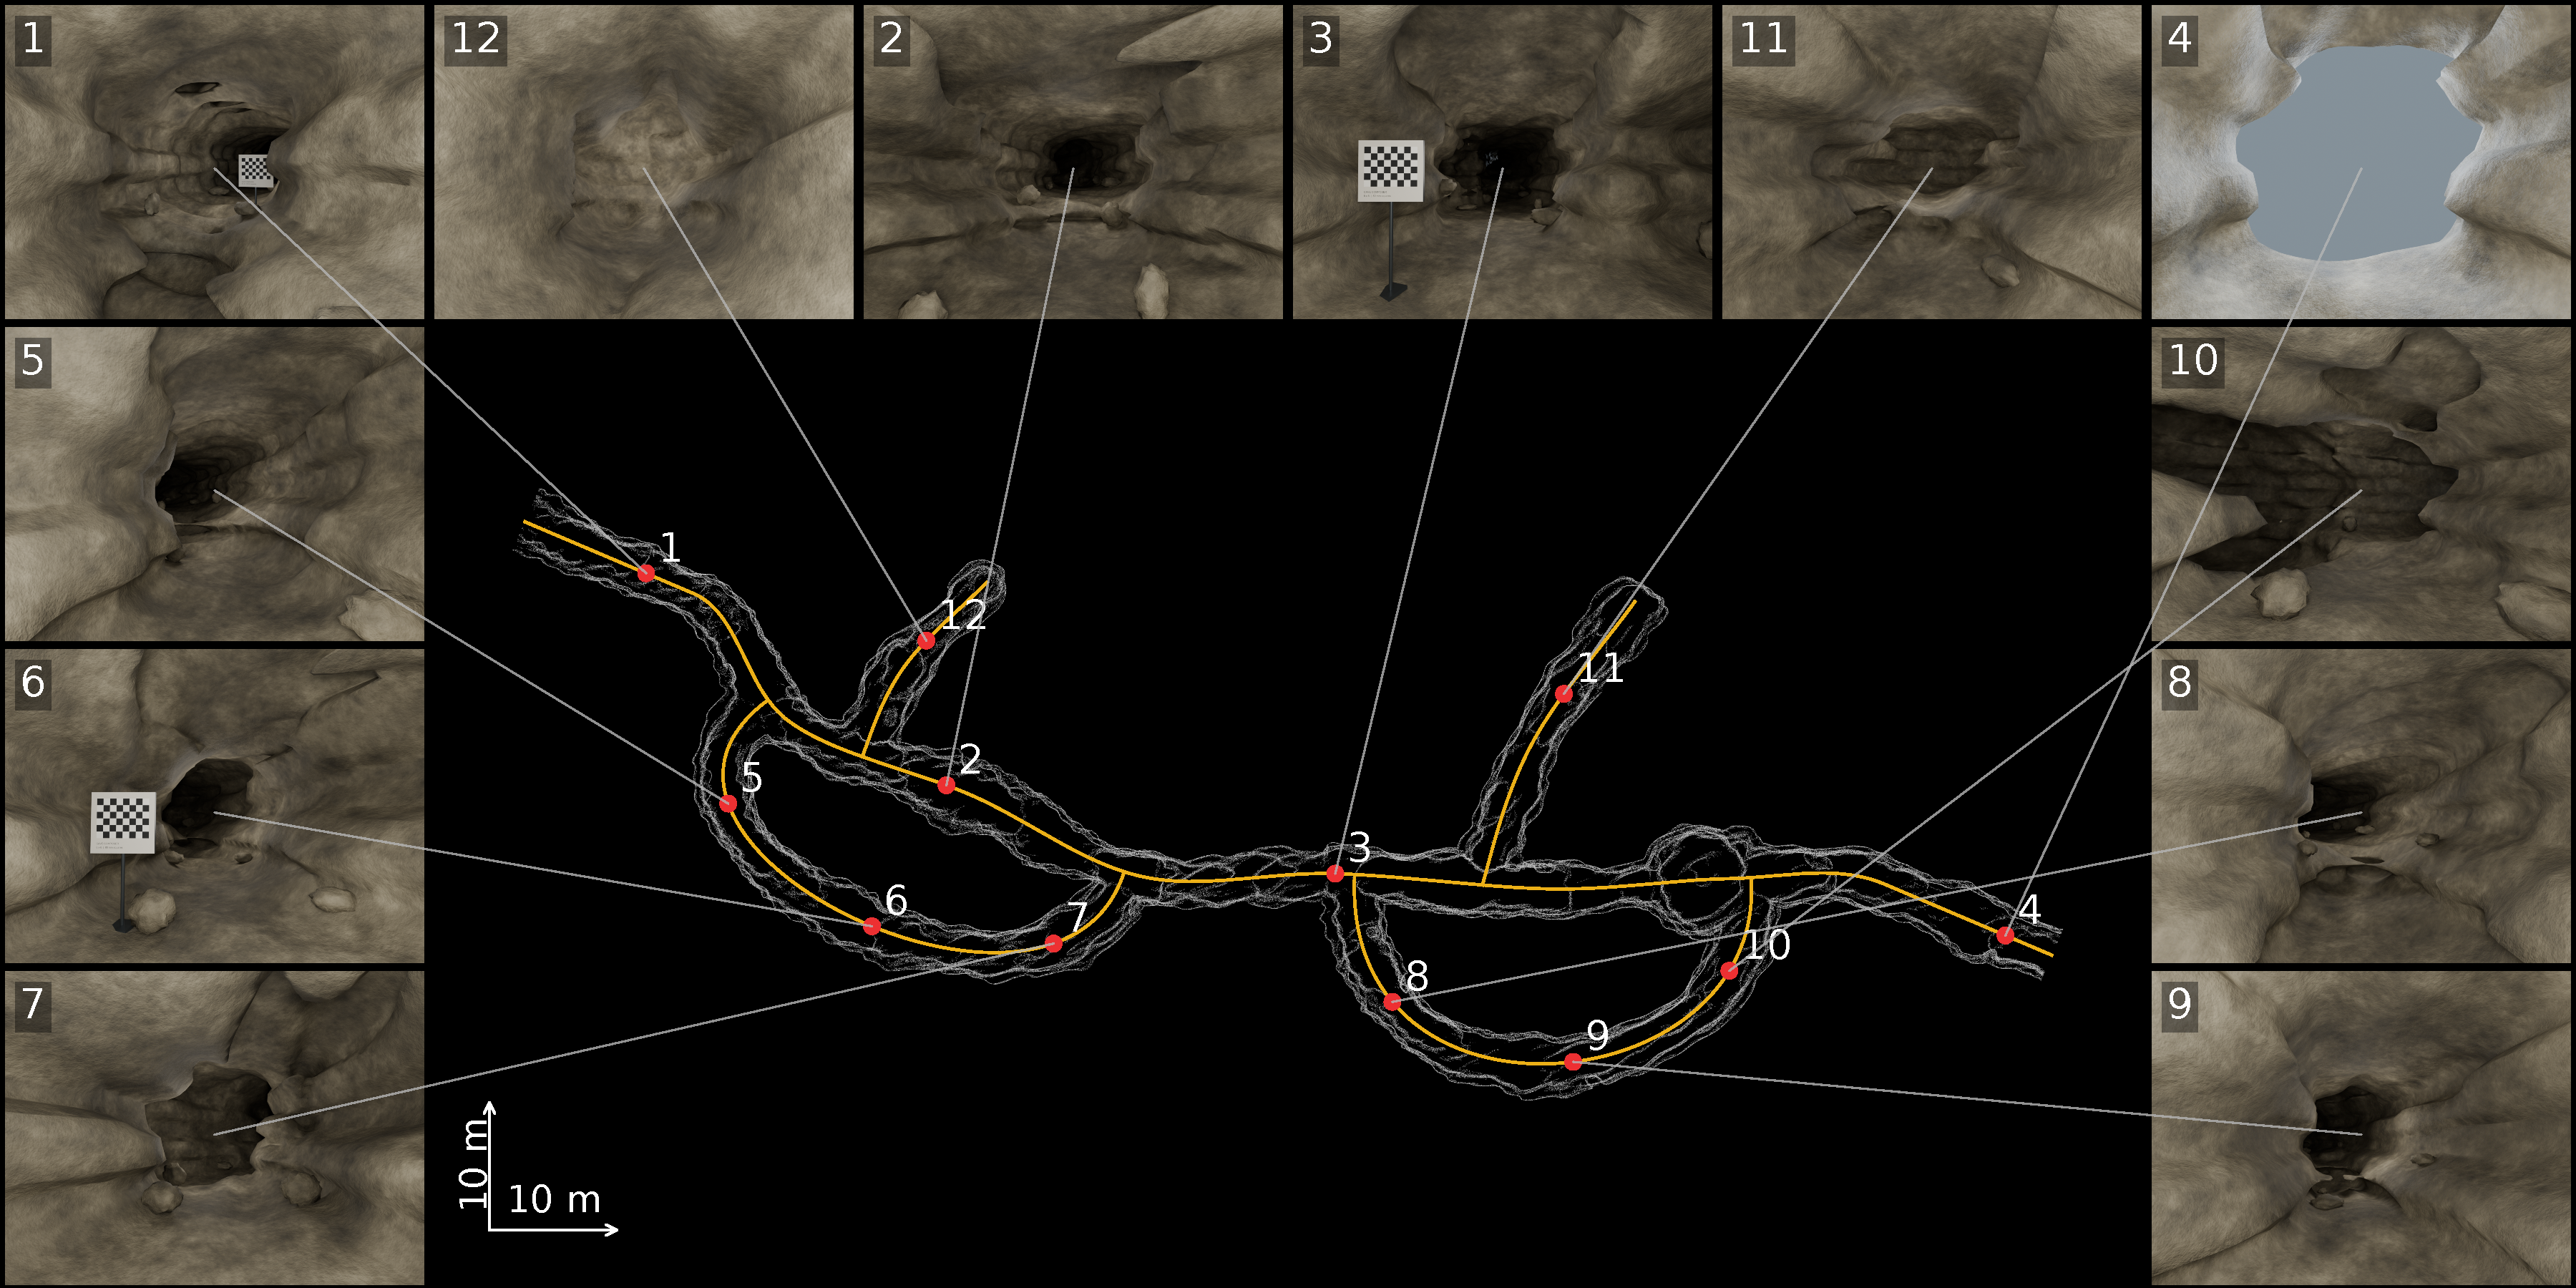
\includegraphics[width=\textwidth]{figures/showcase_hard_v02/cave_showcase.pdf}
\caption{A complex cave generated by Cave Composer, with two rejoining loops
and two blind branches. Twelve Blender interior views are linked to their
camera locations (red) on a mesh-sampled overview; yellow lines show
construction centerlines. Rocks and checkerboard props add local visual detail.
The views use inspection lighting without a water medium. The overview and
centerlines depict generated structure, not a sensor reconstruction or an
executed robot trajectory.}
\label{fig:cave-showcase}
\end{figure*}

The environments used to train a cave-navigation policy determine which
junctions, constrictions and obstacles it encounters, and which failures its
evaluation can reveal. For underwater visual navigation, this makes cave
geometry a central experimental variable alongside sensing and vehicle dynamics.
Changing a passage's shape can simultaneously alter its visual appearance,
occlusion and clearance. If an environment variation blocks the specified robot,
a failed episode no longer isolates the navigation policy's ability to handle
that variation. Conversely, a set of wide, repetitive passages offers limited
coverage of the geometric situations of interest. We study controllable cave
environment generation, with underwater navigation as the motivating application.
Figure~\ref{fig:cave-showcase} illustrates the passage structure and local
appearance of one generated cave.

Procedural generation already supports both environmental diversity and
constraints on usable space. ProcTHOR generates houses and checks agent
reachability after construction~\cite{deitke2022procthor}; Infinigen Indoors
and Holodeck impose constraints on scene composition~\cite{raistrick2024indoors,yang2024holodeck}.
For caves and tunnels, implicit modeling, geological controls and graph-based
authoring provide branching layouts and varied passage
geometry~\cite{raistrick2023infinigen,paris2021caves,cano2024tunnels,garcia2025plume}.
The problem addressed here lies at the intersection of these capabilities:
linking controlled changes in cave structure and local morphology to a specified
robot envelope and start--goal task on the resulting geometry. A desired layout,
a nominal passage width and a path through the final cave describe different
properties; navigation experiments need an explicit relationship between them.

Our central design separates preserving space during generation from establishing
a task's geometric feasibility afterward. A protected passage limits how far
local geometric changes can intrude into the intended route. Surface extraction
and the choice of collision resolution still affect the resulting boundary,
and different endpoint pairs need their own paths. Thus, generation-time
protection supplies a useful construction constraint, while post-generation
checks determine which tasks satisfy the requested clearance on the meshes
actually produced. This separation permits irregular geometry without treating
the generator's own skeleton as evidence of task feasibility.

We introduce \emph{Cave Composer}, a task-conditioned procedural generator for
cave navigation (Fig.~\ref{fig:method}). Structural controls specify turns,
slopes, branches, rejoining passages and chambers; local controls vary sections,
wall intrusions and spatial roughness in an implicit void field. A task sampler
selects multiple start--goal pairs within the same cave. Although construction
routes can guide endpoint selection, the subsequent 3D A* search receives
occupancy and endpoints, not those routes or their graph. Each candidate polyline
is checked for containment and clearance against both extracted visual and
collision meshes, with an allowance for the distance between checked samples.
These checks concern a static spherical envelope on the checked geometry;
dynamic execution and navigation from visual observations are separate questions.

In a paired pilot over six fixed requests, full generation accepts five,
disabling protection accepts four, and restricted generation accepts all six
(Table~\ref{tab:generator}). Protection changes acceptance in one stress case;
another is rejected by both full and unprotected generation. These outcomes
show why acceptance and realized geometric variation must be reported together.
\resultplaceholder{RESULT-GEOM}{State the tested geometric claim,
comparison, independent sample unit, measured result and uncertainty for the
broader generation study.}

Downstream utility concerns the effect of training environments within a fixed
learner and observation setting. A controlled evaluation can use
FlashSAC~\cite{kim2026flashsac} and recurrent visual
PPO~\cite{schulman2017ppo} as separate baselines in an external navigation
platform.
Our contributions are:
\begin{enumerate}
\item We introduce Cave Composer, a controllable cave generator that couples
structural and local geometric variation to robot-dependent passage protection.
Per-task occupancy search and checks on both extracted visual and collision
meshes connect the generated geometry to reproducible navigation tasks.
\item \resultplaceholder{RESULT-NAV}{State the measured effect of training-cave
diversity on held-out navigation performance within each fixed baseline, with
matched observations and training budgets, task definitions and uncertainty.}
\item \resultplaceholder{RESULT-TRANSFER}{State the frozen-policy outcomes on
eligible, previously unseen real-source cave assets in simulation, identifying
task scope, source separation, uncertainty and limitations.}
\end{enumerate}
